% Remote Sensing Letters submission draft (Research Letter, max 12 pages incl. tables and references).
% All table values and \snsm... macros are generated by code_and_results/make_paper_tables.py
% from code_and_results/final/*.csv -- regenerate, never edit numbers by hand.
\documentclass[11pt]{article}
\usepackage[margin=2.5cm]{geometry}
\usepackage{amsmath,amssymb}
\usepackage{graphicx}
\usepackage{booktabs}
\usepackage[T1]{fontenc}
\usepackage{url}
\usepackage{setspace}
\onehalfspacing

\newcommand{\snsmIndianPinesOA}{96.29$\pm$0.74}
\newcommand{\snsmIndianPinesAA}{94.16$\pm$1.07}
\newcommand{\ntrainIndianPines}{505}
\newcommand{\ntestIndianPines}{9744}
\newcommand{\snsmKSCOA}{94.55$\pm$1.25}
\newcommand{\snsmKSCAA}{92.25$\pm$1.84}
\newcommand{\ntrainKSC}{256}
\newcommand{\ntestKSC}{4955}
\newcommand{\snsmPaviaUOA}{99.47$\pm$0.05}
\newcommand{\snsmPaviaUAA}{98.93$\pm$0.16}
\newcommand{\ntrainPaviaU}{2135}
\newcommand{\ntestPaviaU}{40641}
\newcommand{\snsmBotswanaOA}{99.04$\pm$0.69}
\newcommand{\snsmBotswanaAA}{98.85$\pm$1.03}
\newcommand{\ntrainBotswana}{156}
\newcommand{\ntestBotswana}{3092}
\newcommand{\snsmSalinasOA}{99.90$\pm$0.04}
\newcommand{\snsmSalinasAA}{99.86$\pm$0.07}
\newcommand{\ntrainSalinas}{2697}
\newcommand{\ntestSalinas}{50000}
\newcommand{\snsmWHUOA}{99.64$\pm$0.11}
\newcommand{\snsmWHUAA}{99.08$\pm$0.19}
\newcommand{\ntrainWHU}{12868}
\newcommand{\ntestWHU}{50000}
\newcommand{\hybridBWmin}{9.4}


\title{Spectral-neighbourhood self-modulation for lightweight hyperspectral image classification with scarce labels}
\author{Swati Hira$^{a}$\thanks{Corresponding author. Email: shira@iiitn.ac.in},
Devguru Tiwari$^{a}$, Pratibha Kokardekar$^{b}$ and S. R. Sathe$^{c}$\\[4pt]
\small $^{a}$Department of Computer Science and Engineering, IIIT Nagpur, Nagpur, India\\
\small $^{b}$RBU, Nagpur, India; $^{c}$VNIT, Nagpur, India}
\date{}

\begin{document}
\maketitle

\begin{abstract}
\noindent
Lightweight convolutional networks remain attractive for hyperspectral image (HSI) classification when labels are scarce, but their channel-attention blocks usually derive the gating weights from global average pooling followed by fully connected layers, which ignores how statistics vary across neighbouring feature channels. We propose spectral-neighbourhood self-modulation (SNSM), a residual-block modulation in which each channel's scale and shift are predicted by a small one-dimensional convolution over three per-channel descriptors (mean, variance and cross-channel gradient). SNSM adds about 130 parameters per block and is initialised as the identity. Under one fixed protocol (5\% labelled pixels per class, five seeds, 100 epochs, no validation-based model selection) on six benchmark scenes, SNSM reaches \snsmIndianPinesOA\% overall accuracy (OA) and \snsmIndianPinesAA\% average accuracy (AA) on Indian Pines and \snsmKSCOA\% OA on Kennedy Space Center, giving the highest AA among the compared CNN variants and transformer baseline on both scenes. Paired ablations show that the gain comes from the neighbourhood descriptor network rather than from the additive shift: replacing squeeze-and-excitation gating with SNSM gating raises AA by more than 4 points on both scenes, whereas adding the shift changes AA by less than one point. On easier scenes all variants perform alike.
\end{abstract}

\noindent\textbf{Keywords:} hyperspectral image classification; channel attention; feature modulation; few labels; lightweight CNN

\section{Introduction}
Hyperspectral images record hundreds of contiguous bands, which makes pixel-level land-cover classification possible but also exposes classifiers to the Hughes phenomenon when labelled samples are few \cite{hughes1968mean,melgani2004classification}. Convolutional neural networks (CNNs) that operate on spatial--spectral patches are the standard lightweight choice \cite{hu2015deep,makantasis2015deep,li2017spectral,roy2020hybridsn}, while transformer models offer global context at a higher training cost \cite{hong2022spectralformer,sun2022ssftt}.

Channel attention is a cheap way to make a CNN input-dependent. Squeeze-and-excitation (SE) \cite{hu2018squeeze} predicts one scale per channel from globally pooled features through two fully connected (FC) layers; CBAM adds spatial attention \cite{woo2018cbam}; ECA replaces the FC layers by a one-dimensional convolution over the pooled channel vector \cite{wang2020eca}; FiLM adds a shift but takes its conditioning from an external input \cite{perez2018film}. With very few labelled pixels, FC gating has many parameters relative to the training set, and global means alone discard how the response is spread within the patch.

We study a modulation that is (i) local across channels, (ii) driven by several per-channel statistics rather than the mean only, and (iii) identity at initialisation. Our contributions are:
\begin{itemize}
\item SNSM, a residual-block modulation whose scale and shift come from a dilated one-dimensional convolution over normalised channel means, variances and cross-channel gradients (Section~\ref{sec:method});
\item a single-protocol comparison on six scenes in which every model, including HybridSN and SSFTT, is trained on the same splits, inputs and schedule with no validation-based checkpoint selection (Section~\ref{sec:setup});
\item paired same-seed ablations that separate the effect of the descriptor network from the effect of the additive shift (Section~\ref{sec:results}).
\end{itemize}

\section{Method}\label{sec:method}
\subsection{Input features}
Each band of the raw cube is smoothed with a $5\times5$ adaptive Wiener filter. Principal component analysis (PCA) then reduces the spectrum to 30 components; it is fitted without labels on all pixels of the scene. A one-level db4 discrete wavelet transform \cite{daubechies1992ten} is applied to each component, and its approximation sub-band, resized bilinearly to the image size, is concatenated with the components, giving $B=60$ features per pixel. Each labelled pixel is represented by the $15\times15\times B$ patch centred on it (zero padding at the image border).

\subsection{Backbone}
A $3\times3$ convolution maps the $B$ input features to $C=64$ channels (batch normalisation, ReLU). Two residual blocks follow, each computing
\begin{equation}
\mathbf{h}=\mathrm{ReLU}(\mathrm{BN}(\mathrm{Conv}_{3\times3}(\mathbf{x}))),\qquad
\mathbf{y}=\mathrm{ReLU}\big(\mathrm{BN}(\mathrm{Conv}_{3\times3}(\mathcal{M}(\mathbf{h})))+\mathbf{x}\big),
\end{equation}
where $\mathcal{M}$ is the modulation under study ($\mathcal{M}=$ identity for the plain CNN). Global average pooling, dropout (0.4) and a linear layer produce the class scores.

\subsection{Spectral-neighbourhood self-modulation}
For $\mathbf{h}\in\mathbb{R}^{C\times H\times W}$, SNSM first computes three descriptors for every channel $c$: the spatial mean $\mu_c$, the spatial variance $v_c$, and the cross-channel gradient $g_c=(\mu_{c+1}-\mu_{c-1})/2$ (one-sided differences at the first and last channel). Each descriptor vector is standardised across channels, $\tilde{s}=(s-\bar{s})/(\sigma_s+\epsilon)$, and the three are stacked into $\mathbf{S}\in\mathbb{R}^{3\times C}$. Two one-dimensional convolutions along the channel axis give
\begin{equation}
\mathbf{Z}=\mathrm{Conv1D}^{(2)}_{k=3}\big(\mathrm{ReLU}(\mathrm{Conv1D}^{(1)}_{k=3,\,d=2}(\mathbf{S}))\big)\in\mathbb{R}^{2\times C},
\end{equation}
with 8 hidden channels, dilation $d=2$ in the first layer and replicate padding. The modulation is
\begin{equation}
\gamma_c=1+\tfrac12\tanh(Z_{1,c}),\qquad \beta_c=Z_{2,c},\qquad \mathcal{M}(\mathbf{h})_c=\gamma_c\,\mathbf{h}_c+\beta_c .
\end{equation}
The weights and bias of $\mathrm{Conv1D}^{(2)}$ are initialised to zero, so every block starts as the plain residual block and $\gamma_c\in[0.5,1.5]$ thereafter. The modulation adds 130 parameters per block, against 2{,}128 for SE gating with reduction to 16 units. Each channel's parameters depend on a window of neighbouring channels (receptive field of seven channels), as in ECA \cite{wang2020eca}; unlike ECA, SNSM uses dispersion and gradient descriptors in addition to the mean, outputs a shift as well as a scale, and starts from the identity. The SNSM ($\gamma$) variant drops the shift output.

\section{Experimental setup}\label{sec:setup}
\textbf{Data.} We use Indian Pines (IP), Pavia University (PU), Kennedy Space Center (KSC), Botswana (BW), Salinas and WHU-Hi HanChuan \cite{baumgardner2015indian,gamba2004pavia,gic2020hyperspectral,zhong2020whu}. For each class, 5\% of the labelled pixels (at least one) are drawn at random for training and the remaining labelled pixels are used for testing; for Salinas and WHU-Hi a random subset of 50{,}000 test pixels is used. This gives \ntrainIndianPines/\ntestIndianPines\ (IP), \ntrainKSC/\ntestKSC\ (KSC), \ntrainPaviaU/\ntestPaviaU\ (PU) and \ntrainBotswana/\ntestBotswana\ (BW) training/test pixels.

\textbf{Models.} On IP, KSC, PU and BW we compare six modulation variants on the same backbone (plain CNN; SE ($\gamma$) \cite{hu2018squeeze}; ECA ($\gamma$) \cite{wang2020eca}, with kernel size 3 as given by its adaptive rule for 64 channels; FC ($\gamma{+}\beta$), i.e.\ SE-style FC layers predicting a sigmoid scale and a linear shift; SNSM ($\gamma$); SNSM ($\gamma{+}\beta$)) with HybridSN \cite{roy2020hybridsn} in its original layer configuration. SSFTT \cite{sun2022ssftt} (four tokens, one transformer layer with eight heads) is reimplemented and run on IP and KSC only. Salinas and WHU-Hi are near saturation and are run with SNSM only.

\textbf{Protocol.} Every model sees the same 60-feature patches and the same splits for a given seed. Training uses cross-entropy, AdamW \cite{loshchilov2019decoupled} (learning rate $10^{-3}$, weight decay $10^{-4}$), a step decay (factor 0.5 every 40 epochs), batch size 64 and exactly 100 epochs, with no data augmentation and no early stopping. The final-epoch model is evaluated once; no validation or test data are used for model selection. Each configuration is repeated with seeds 42--46, and we report mean $\pm$ sample standard deviation. Runs used PyTorch \cite{paszke2019pytorch} on an NVIDIA Tesla T4. Baselines are therefore trained under our protocol and inputs rather than their original settings, so their accuracies are not directly comparable to published values.

\section{Results}\label{sec:results}
\begin{table}[t]
\caption{OA and AA (\%, mean $\pm$ std over five seeds) at 5\% labelled pixels. Best mean per column in bold.}
\label{tab:main}
\centering\small
\resizebox{\textwidth}{!}{\begin{tabular}{lcccccccc}
\toprule
Method & \multicolumn{2}{c}{IP} & \multicolumn{2}{c}{KSC} & \multicolumn{2}{c}{PU} & \multicolumn{2}{c}{BW} \\
 & OA & AA & OA & AA & OA & AA & OA & AA \\
\midrule
Plain CNN & 95.96$\pm$0.89 & 87.86$\pm$1.29 & 90.93$\pm$6.94 & 85.64$\pm$12.98 & \textbf{99.59$\pm$0.07} & \textbf{99.01$\pm$0.16} & 99.09$\pm$0.55 & 98.87$\pm$0.90 \\
SE ($\gamma$) & 96.23$\pm$0.69 & 89.49$\pm$2.39 & 91.54$\pm$5.56 & 87.32$\pm$8.36 & 99.53$\pm$0.19 & 98.80$\pm$0.56 & 98.95$\pm$0.82 & 98.76$\pm$1.07 \\
FC ($\gamma{+}\beta$) & 96.24$\pm$0.52 & 92.51$\pm$1.60 & 84.31$\pm$6.34 & 77.25$\pm$8.18 & 99.51$\pm$0.06 & 98.88$\pm$0.14 & 98.80$\pm$0.70 & 98.63$\pm$0.98 \\
SNSM ($\gamma$) & 96.19$\pm$0.74 & 93.70$\pm$1.38 & 94.49$\pm$2.02 & 91.63$\pm$3.04 & 99.49$\pm$0.05 & 98.91$\pm$0.16 & \textbf{99.10$\pm$0.62} & \textbf{98.89$\pm$0.96} \\
SNSM ($\gamma{+}\beta$) & 96.29$\pm$0.74 & \textbf{94.16$\pm$1.07} & \textbf{94.55$\pm$1.25} & \textbf{92.25$\pm$1.84} & 99.47$\pm$0.05 & 98.93$\pm$0.16 & 99.04$\pm$0.69 & 98.85$\pm$1.03 \\
\midrule
HybridSN & 88.30$\pm$4.91 & 73.64$\pm$8.28 & 68.04$\pm$9.32 & 55.19$\pm$11.33 & 97.84$\pm$1.52 & 95.46$\pm$4.12 & 77.16$\pm$37.92 & 75.56$\pm$38.31 \\
SSFTT & \textbf{96.71$\pm$0.79} & 92.35$\pm$1.81 & 80.44$\pm$2.57 & 68.50$\pm$3.65 & -- & -- & -- & -- \\
\bottomrule
\end{tabular}
}
\end{table}

\textbf{Accuracy.} Table~\ref{tab:main} gives the main comparison. On IP, SNSM ($\gamma{+}\beta$) has the highest AA; SSFTT has the highest OA but a lower AA. On KSC, SNSM ($\gamma{+}\beta$) has the highest OA and AA, and its seed-to-seed spread is several times smaller than that of the plain and SE models. On PU and BW the six CNN variants are within a few tenths of a point of each other (the plain CNN is marginally best on PU), so modulation brings no measurable benefit on these scenes. HybridSN trained under our protocol is less accurate and less stable; on one BW seed it did not converge (\hybridBWmin\% OA). SNSM reaches \snsmSalinasOA\% OA on Salinas and \snsmWHUOA\% OA on WHU-Hi.

\begin{table}[t]
\caption{Paired same-seed differences in AA (percentage points): mean over five seeds and number of seeds with a positive difference.}
\label{tab:paired}
\centering\small
\begin{tabular}{lcccc}
\toprule
$\Delta$AA (wins/5) & IP & KSC & PU & BW \\
\midrule
SNSM ($\gamma{+}\beta$) $-$ SNSM ($\gamma$) & +0.46 (3/5) & +0.62 (3/5) & +0.02 (3/5) & -0.03 (1/5) \\
FC ($\gamma{+}\beta$) $-$ SE ($\gamma$) & +3.02 (5/5) & -10.07 (0/5) & +0.09 (1/5) & -0.13 (1/5) \\
SNSM ($\gamma$) $-$ SE ($\gamma$) & +4.22 (5/5) & +4.31 (4/5) & +0.11 (1/5) & +0.13 (2/5) \\
SNSM ($\gamma{+}\beta$) $-$ Plain CNN & +6.30 (5/5) & +6.60 (4/5) & -0.08 (2/5) & -0.01 (2/5) \\
\bottomrule
\end{tabular}

\end{table}

\textbf{Where the gain comes from.} Table~\ref{tab:paired} pairs runs that share a seed and therefore a split. Replacing SE gating by the SNSM descriptor network (both scale-only) raises AA on IP and KSC in nine of ten paired runs, with mean gains above 4 points. ECA, which also gates each channel with a local convolution across channels but uses only the channel mean, has lower AA than SNSM ($\gamma$) on IP (four of five seeds) and KSC (three of five seeds, with a large seed-to-seed spread for ECA), so locality across channels alone does not explain the gain; we did not separate the contributions of the extra descriptors and of the identity initialisation. Adding the shift to SNSM changes AA by less than one point and helps in only three of five seeds on either scene, so we do not claim a benefit from the shift itself. Adding a shift to FC gating helps on IP but lowers AA by about 10 points on KSC, which suggests that an unconstrained FC shift is unstable with 256 training pixels, whereas SNSM's bounded scale and zero-initialised output avoid this.

The AA gains on IP come from small classes. Relative to the plain CNN, SNSM ($\gamma{+}\beta$) raises mean per-class accuracy on Oats (20 labelled pixels) from 21.1\% to 74.7\%, on Grass-pasture-mowed (28) from 63.0\% to 92.6\%, and on Stone-Steel-Towers (93) from 76.9\% to 92.4\%. On KSC the largest change is for Cabbage palm hammock, from 60.3\% to 93.1\%.

\begin{figure}[t]
\centering
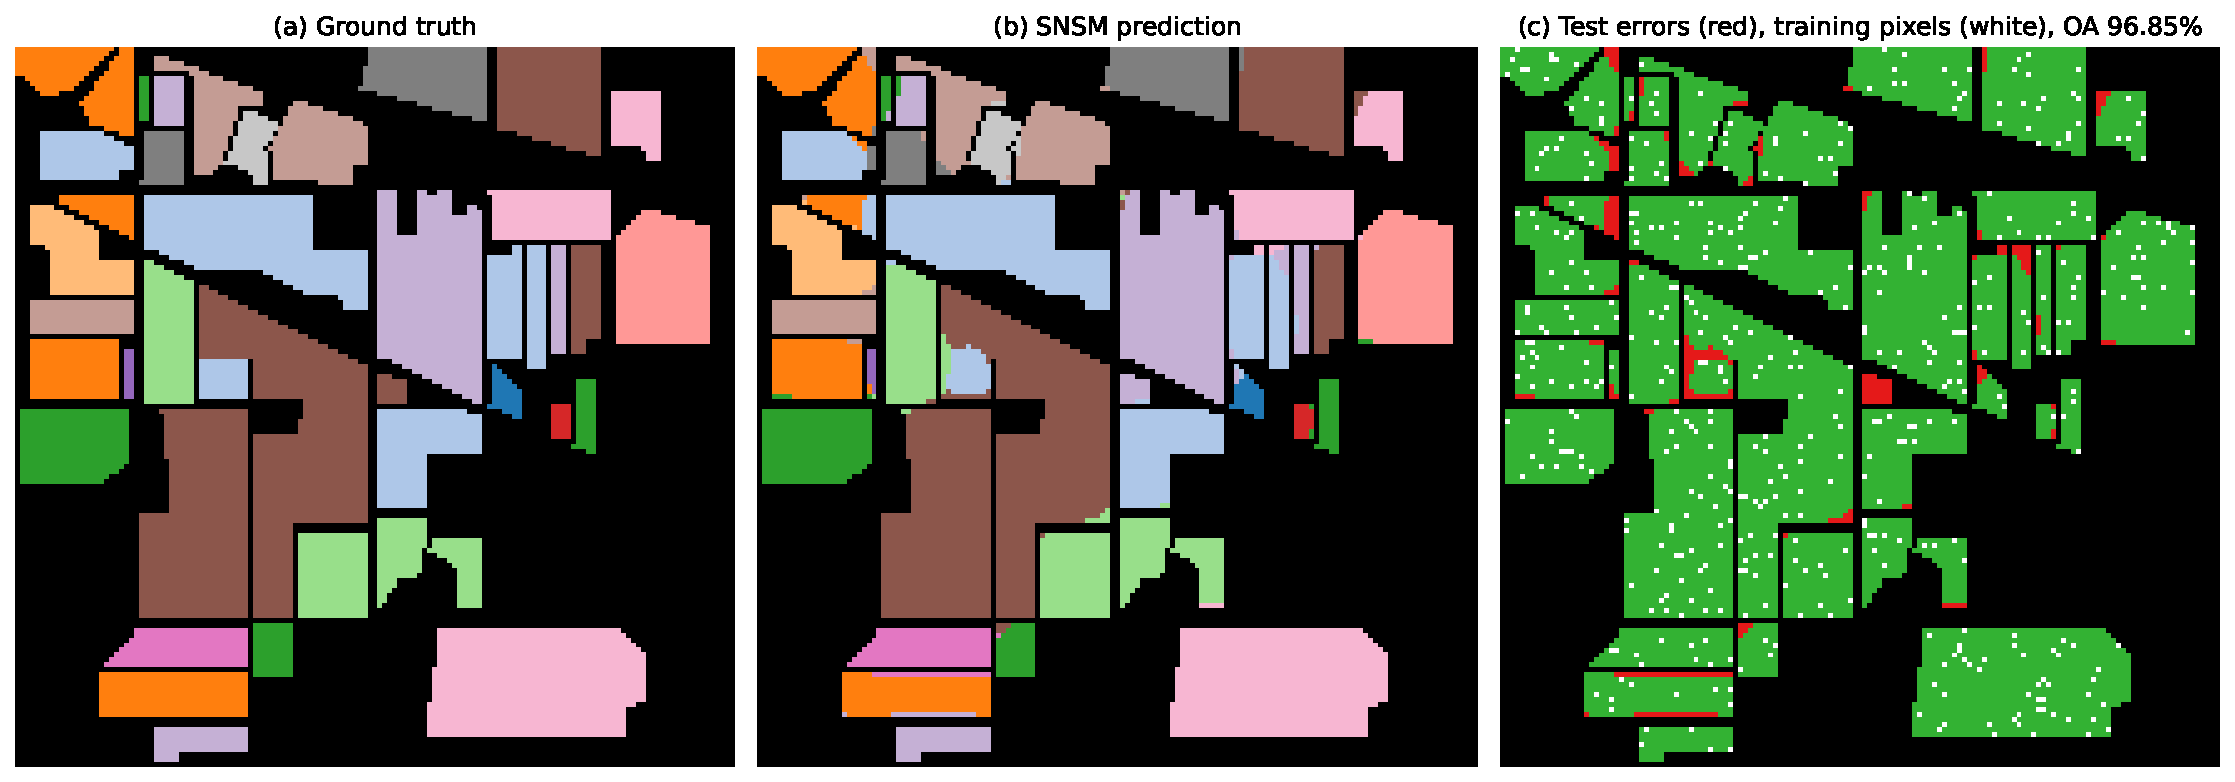
\includegraphics[width=\textwidth]{../../code_and_results/final/classification_map_IndianPines.pdf}
\caption{Indian Pines, SNSM ($\gamma{+}\beta$), seed 42: (a) ground truth, (b) prediction for all labelled pixels, (c) test errors in red and training pixels in white.}
\label{fig:map}
\end{figure}

\begin{table}[t]
\caption{Model size and cost for a $15\times15\times60$ IP patch. $^{a}$Multiply--accumulates of convolution and linear layers counted by \texttt{thop}; tensor operations such as attention products and descriptor statistics are not included. $^{b}$Batch size 1 on a Tesla T4. Training time is the mean per run (100 epochs).}
\label{tab:eff}
\centering\small
\begin{tabular}{lrrrrr}
\toprule
Method & Params (M) & MMACs$^{a}$ & Latency (ms)$^{b}$ & Train IP (s) & Train PU (s) \\
\midrule
Plain CNN & 0.184 & 41.2 & 0.69 & 4.4 & 17.6 \\
SE ($\gamma$) & 0.188 & 41.2 & 1.17 & 4.6 & 19.3 \\
FC ($\gamma{+}\beta$) & 0.190 & 41.2 & 1.31 & 4.7 & 19.8 \\
SNSM ($\gamma$) & 0.184 & 41.3 & 2.54 & 7.5 & 29.5 \\
SNSM ($\gamma{+}\beta$) & 0.184 & 41.3 & 2.54 & 7.6 & 30.2 \\
HybridSN & 1.743 & 137.4 & 0.71 & 26.2 & 115.3 \\
SSFTT & 0.291 & 34.9 & 1.25 & 7.6 & -- \\
\bottomrule
\end{tabular}

\end{table}

\textbf{Cost.} SNSM adds almost no parameters or multiply--accumulates to the plain CNN (Table~\ref{tab:eff}), but its descriptor computation consists of many small operations, so batch-1 latency and training time are higher than for the plain and SE models. All CNN variants remain an order of magnitude smaller than HybridSN.

\section{Discussion and limitations}
Local cross-channel modulation helps where it is most needed: scenes with small, spectrally similar classes (IP, KSC), and it does so with fewer gating parameters than SE. Its benefit disappears on scenes where a plain CNN is already near saturation. Several limitations apply. Training and test pixels are drawn at random from the same scene, so overlapping patches share spatial context and accuracies are optimistic compared with spatially disjoint splits. PCA is fitted on all pixels of each scene without labels. Five seeds give only an indication of variability, and the paired differences in Table~\ref{tab:paired} are not formal significance tests. Baselines were not tuned to our protocol, and CBAM was not included in the unified comparison. Finally, the channel order of learned feature maps has no physical wavelength meaning, so ``neighbourhood'' refers to adjacency of feature channels, which the first convolution is free to learn.

\section{Conclusion}
SNSM predicts per-channel scale and shift with a small convolution over neighbouring channels' mean, variance and gradient. Under a single strict protocol it gives the best average accuracy on Indian Pines and KSC at 5\% labels with about 130 extra parameters per block. Paired ablations attribute the improvement to the neighbourhood descriptor network rather than to the additive shift.

\section*{Disclosure statement}
The authors report there are no competing interests to declare.

\section*{Funding}
No external funding was received for this research.

\section*{Data and code availability}
The datasets are publicly available \cite{gic2020hyperspectral,zhong2020whu}. Code, per-run results and the scripts that generate every table are available at \url{https://github.com/Devguru-codes/research_paper_code}.

\section*{Use of generative AI}
% TODO(authors): confirm or edit this statement before submission.
Generative AI (Claude, Anthropic) was used to help write and check experiment code and to draft and edit the text. The authors reviewed all outputs and take full responsibility for the content.

\bibliographystyle{plain}
\bibliography{../sn-bibliography}

\end{document}
